
\chapter{Metodologia} \label{cap:metodos}
    Em resumo a metodologia experimental deste trabalho consiste nos seguintes passos:
    \begin{itemize}
        \item Coleta de dados endógenos e exógenos
        \item Transformação de cada registro de dado endógeno (os dados de consumo e vendas), em uma série temporal com intervalo de 5 dias anteriores.
        \item Analises exploratórias dos conjuntos de dados endógenos e exógenos com o conjunto de dados a serem previstos.
        \item Construção e treino dos modelos exclusivamente endógenos e dos modelos mistos, duplicados em 2 fases experimentais com diferentes domínios temporais.
        \item Analises comparativas dos resultados dos modelos.
        \item Conclusões sobre os resultados e seleção do melhor modelo.
    \end{itemize}
    
	\section{Pré-processamento}
	    Na etapa de pre-processamento dos dados, além da obtenção dos dados, também é realizada a etapa de transformação dos dados em séries temporais, normalização com a remoção de outliers, e aplicação da escala 0 a 1, para que todos os dados correspondam à um mesmo domínio de aprendizado.
	    Após a conclusão destas etapas o conjunto de dados foi preparado para as fases experimentais 1 e 2, que realizaram uma divisão do conjunto final de dados em intervalos temporais distintos.
	    
	    \subsection{Dados endógenos}
        	Os dados históricos de consumo no restaurante foram retirados do atual sistema banco de dados de refeições subsidiadas do Hospital São Paulo, que gerencia os dados dos refeitórios de todos as unidades da Unifesp.
        	
        	Apenas alguns funcionários autorizados tem acesso ao banco de dados do sistema de refeições da instituição, entre eles o fiscal de contrato do restaurante universitário. Para obter tais dados neste trabalho, foi necessário obter uma autorização com a direção do campus ICT - UNIFESP e em seguida solicitar a exportação dos dados ao fiscal. Para este trabalho foram solicitados os dados de consumo exclusivamente de alunos, pois podem ser obtidos também os dados de professores, alunos de pós-graduação e visitantes. 
    
        	\begin{table}[!ht]
        	    \centering
                \rowcolors{2}{gray!25}{white}
                \begin{tabular}{|l|l|l|}
                    \hline
                    DATA                  & (19/12/2017) & (18/12/2017) \\ \hline
                    VENDAS CAFÉ           & 0            & 0            \\
                    VENDAS ALMOÇO         & 24           & 71           \\
                    VENDAS JANTAR         & 0            & 0            \\
                    VENDAS REFEIÇÃO*      & 24           & 71           \\
                    TOTAL VENDAS          & 24           & 71           \\
                    ENTR. CAFÉ            & 0            & 0            \\
                    ENTR. ALMOÇO          & 42           & 70           \\
                    ENTR. JANTAR          & 3            & 24           \\
                    TOTAL ENTR. REFEIÇÃO* & 45           & 94           \\
                    TOTAL ENTRADA         & 45           & 94           \\ \hline
                \end{tabular}
                \caption{Formato dos dados originais obtidos pelo restaurante universitário}
                \label{table:dadosrestaurante}
            \end{table}
            Os dados exportados pelo sistema do restaurante da Unifesp foram obtidos de acordo com o formato da tabela \ref{table:dadosrestaurante}\\
            
            \begin{table}[!ht]
                \centering
                \rowcolors{2}{gray!25}{white}
                \begin{tabular}{|l|l|}
                \hline
                    DATA                  & (19/12/2017) \\ \hline
                1 DIA ANTERIOR    & 500        \\
                2 DIAS ANTERIORES & 00                            \\
                3 DIAS ANTERIORES & 300                            \\
                4 DIAS ANTERIORES & 200                            \\
                5 DIAS ANTERIORES & 100                          \\ \hline 
                \end{tabular}
                \caption{Transformação dos registros do restaurante em uma série temporal}
                \label{table:transformacaodadosrestaurante}
            \end{table}
            
            Após a coleta, os dados de consumo do restaurante foram transformados em um processo de aproximação por uma série temporal, para um intervalo de 5 dias, e em cada registro de venda são acrescentados 5 novos atributos contendo os valores passados, deste mesmo atributo, em um intervalo de 5 dias anteriores. Este processo adapta o conjunto de dados para o processo de memorização das entradas, estruturando o formato compatível de leitura de dados nos modelos de redes neurais desenvolvidos. A tabela \ref{table:transformacaodadosrestaurante} representa a nova estrutura de um registro de dado do restaurante, com um intervalo temporal de 5 dias anteriores. Nota-se que o valor de consumo da data 20/04/2017 foi removido do conjunto de dados, por se tratar o valor supervisionado a ser previsto, dado que o processo de aprendizado das redes neurais utilizam apenas dados no passado, a partir de 1 dia anterior.
            
           
        \subsection{Dados exógenos}
            Os dados exógenos correlacionados com o consumo se dividem em 2 tipos principais, os dados climáticos coletados de estações meteorológicas próximas ao ICT Unifesp, e dados derivados das datas dos registros de consumo.
            
            \paragraph{Dados Climáticos}
            	Também obteve-se variáveis climáticas como dados exógenos, para a influência de fatores externos (temperatura média ambiente, pressão atmosférica, umidade e velocidade do vento). Tais dados podem ser obtidos de forma gratuita pelo BDMEP - Banco de Dados Meteorológicos para Ensino e Pesquisa, pertencente à instituição pública INMET - Instituto Nacional de Meteorologia, pertencente ao MINISTÉRIO DA AGRICULTURA, PECUÁRIA E ABASTECIMENTO do Governo Brasileiro. 
            	
            	É necessário um cadastro no site http://www.inmet.gov.br/portal/index.php?r=bdmep/bdmep para a obtenção dos dados. 
            	
            	A instituição contêm dados registrados de forma digital desde 1961 no país inteiro, os dados históricos referentes a períodos anteriores a 1961 ainda não estão em forma digital e, portanto, estão indisponíveis no BDMEP.
            	
            	Importante ressaltar que o BDMEP leva 90 dias para registrar cada nova data.
            	
        	\paragraph{Dados de Calendário}
            	A informação de data contida nos índices dos registros dos dados endógenos, foi derivada em diversas informações que representam o comportamento de consumo em relação à sazonalidade da frequência dos alunos influenciada pelas agendas de atividades acadêmicas.\\
            	Os seguintes parâmetros foram definidos:
            	\begin{itemize}
            	    \item Semestre 1 ou 2 em formato categórico e binário.
            	    \item Dia da semana em formato categórico e binário.
            	    \item Distancia em dias até o registro anterior e posterior.
            	    \item Avanço do semestre em escala percentual.
            	    \item Avanço do mês em escala percentual.
            	\end{itemize}
            	
            	O dia da semana seguiu o modelo binário de acordo com os trabalho de previsão de demanda em R.U realizados por \cite{Lopes2008} e \cite{Rocha2011}.
        
                \begin{figure}[H]
                	\center{
                		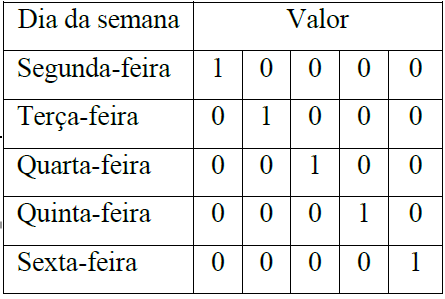
\includegraphics[width=0.40\textwidth]
                		{04-lopes-entradas-dia-semana.png}
                	\caption{Entradas de dia da semana em cofatores.} \subcaption*{ Retirado de \cite{Lopes2008}.}\label{fig:entradasSemanais}}
                \end{figure}
                
	\subsection{Formato final do conjunto de dados}
       \begin{table}[!ht]
            \centering
            \rowcolors{2}{gray!25}{white}
            \begin{tabular}{|c|c|c|} \hline
                \multicolumn{3}{c}{ Estrutura final do conjunto de dados indexados por data: } \\
                \hline
                identificador &	nome da variável					&tipo de variável\\ 
                \hline
                0&	SEMESTRE\_1					&int64 \\
                1&	SEMESTRE\_2					&int64\\
                2&	SEGUNDA						&int64 \\
                3&	TERCA						&int64 \\
                4&	QUARTA						&int64 \\ 
                5&	QUINTA						&int64 \\ 
                6&	SEXTA						&int64 \\ 
                7&	DISTANCIA\_DIA\_ANTERIOR	&	int64 \\ 
                8&	DISTANCIA\_DIA\_POSTERIOR	&	int64 \\
                9&	PERC\_CONCLUSAO\_SEM		&	float64 \\
                10&	PERC\_CONCLUSAO\_MES		&	float64 \\
                11&	PRESSAO\_ATMOSFERICA		&	float64 \\
                12&	TEMPERATURA					&float64 \\ 
                13&	UMIDADE						&int64 \\
                14&	VENTO						&float64\\ 
                15&	VENDAS\_ALMOCO				&int64 \\
                16&	VENDAS\_ALMOCO\_1			&	int64 \\ 
                17&	VENDAS\_ALMOCO\_2			&	int64 \\
                18&	VENDAS\_ALMOCO\_3			&	int64\\ 
                19&	VENDAS\_ALMOCO\_4			&	int64 \\
                20&	VENDAS\_ALMOCO\_5			&	int64 \\ 
                21&	ENTR\_ALMOCO				&	int64\\
                22&	ENTR\_ALMOCO\_1				&int64 \\
                23&	ENTR\_ALMOCO\_2				&int64 \\
                24&	ENTR\_ALMOCO\_3				&int64 \\ 
                25&	ENTR\_ALMOCO\_4				&int64 \\
                26&	ENTR\_ALMOCO\_5				&int64 \\
                27&	ENTR\_JANTAR				&	int64 \\ 
                28&	ENTR\_JANTAR\_1				&int64\\
                29&	ENTR\_JANTAR\_2				&int64 \\ 
                30&	ENTR\_JANTAR\_3				&int64 \\ 
                31&	ENTR\_JANTAR\_4				&int64 \\
                32&	ENTR\_JANTAR\_5				&int64\\
              \hline
            \end{tabular}
            \caption{Estrutura final do conjunto de dados indexados por data}
            \label{table:dataset_final}
        \end{table}
        Por fim, a tabela \ref{table:dataset_final} representa o conjunto de dados estruturados e preparados para o processo de divisão em domínios de treino, validação e teste para o treino dos modelos.
        
        \subsection{Tratamento dos dados para entrada nos modelos}
         	Os dados endógenos, após estruturados na tabela final do conjuntos de dados, ainda passam pelas seguintes transformações:
         	\begin{itemize}
                \item	Calculo do desvio padrão de cada vetor de atributos, e normalização dos valores máximos para o teto de 3x o desvio padrão, e mínimo de 0. 
                \item	Transformação dos dados em escala de 0 e 1
            \end{itemize}
            Os dados exógenos não passam pela transformação em série temporal, portanto os mesmos são tratados de acordo com os passos:
            \begin{itemize}
                \item	Transformação dos dados em escala de 0 e 1.
                \item	Os parâmetros categóricos binários (dias da semana e semestre) já estão escalados por serem categorias binárias.
            \end{itemize}
    	\subsection{Fases Experimentais}
            O processo experimental é realizado em 2 roteiros distintos de divisão do domínio temporal do conjunto de dados, e os resultados obtidos entre as duas fases serão comparados.
            
            O conjunto de dados contemplando o período de 2017 a 2019, é dividido em conjunto de treino, validação e teste da seguinte maneira: 
            
            \paragraph{1º Fase com validação no 1º semestre de 2018 e teste no 1º semestre de 2019}
                Neste roteiro o semestre de validação que compõe o conjunto de dados para o treino backpropagation das redes neurais, contempla o primeiro semestre de 2018 e o conjunto de teste contempla o primeiro semestre de 2019.
                Os dados de 2017 contemplando o 1º e 2º semestre, e 2018 contemplando o 2º semestre, são usados para treino. Os resultados obtidos nesta divisão são usados para validar a hipótese de que os modelos aprendem especificamente a sazonalidade de consumo no primeiro semestre, se saindo melhor nos testes realizados no primeiro semestre de 2019, em comparação aos outros modelos treinados com validação no ano todo de 2018.
                Portanto o conjunto de dados da primeira fase contempla o seguinte domínio:
            \begin{itemize}
                    \item Conjunto de treino dos modelos, contemplando o primeiro e segundo semestre de 2017, e segundo semestre de 2018.
                    \item Conjunto de validação dos modelos, contemplando o primeiro semestre de 2018.
                    \item Conjunto de teste dos modelos, contemplando o primeiro semestre de 2019             
            \end{itemize}
            
            \paragraph{2º Fase com treino em 2017, validação em 2018 e teste em 2019}
                Nesta fase, os conjuntos são divididos conforme sua descrição, e o melhor modelo encontrado passa por uma última etapa de teste no domínio da primeira fase (teste somente no primeiro semestre de 2019).
                As métricas obtidas neste teste são comparadas com o melhor modelo da primeira fase.
    
    \section{Definição e treino dos modelos}
        \subsection{Topologia}
            \paragraph*{Sobre a necessidade de se implementar modelos mistos}
                No conjunto de dados deste trabalho, os dados obtidos se dividem em dados temporais (onde cada registro de consumo e venda trás a informação de seu domínio em um intervalo de 5 dias anteriores) e dados discretos onde temos variáveis categóricas de data para cada registro, e variáveis climáticas, porém sem a aplicação de um intervalo temporal, ou seja, os dados exógenos são discretos, e os endógenos são temporais.
                Portanto é necessária a implementação de modelos específicos para entradas temporais e modelos específicos para as entradas discretas.
                Para a saída final foi implementado um comitê de redes neurais endógenas e exógenas, com um perceptron na saída, recebendo os 2 valores dos modelos endógenos e exógenos para a regressão das saídas das 2 redes ao valor que será a predição do consumo.
         	\subsubsection{Modelos endógenos}
         	\begin{itemize}
                \item	Desenvolvimento das redes perceptron de baixa profundidade para avaliar o aprendizado da rede
                \item	Aumento da profundidade da rede e avaliar as mudanças da função de perda RMSE. 
                \item	Implementação e avaliação dos modelos com redes recorrentes GRU, conforme a figura \ref{fig:gru-arch} que são especialmente desenvolvidos para o aprendizado com memorização de dados, e no caso deste trabalho, podem memorizar as sazonalidades semanais de consumo (em um intervalo de 5 dias).
            \end{itemize}
            \subsubsection{Modelos Mistos : Endógenos e Exógenos}
                \begin{itemize}
                    \item Para os dados temporais (consumo e venda) utilizou-se os melhores modelos endógenos dos experimentos anteriores para as entradas endógenas. 
                    \item Para os dados discretos e categóricos adaptou-se a entrada destes dados para rede perceptron
                    \item  Concatenou-se a saída das 2 redes neurais em um percetron criando um comitê de redes neurais para obter a saída final prevista.
                \end{itemize}
                %TODO-T: FIGURA 24 ESTORANDO MARGEM DO TITULO
	\subsection{Função de ativação}
	    \begin{figure}[H]
        	\center{
        		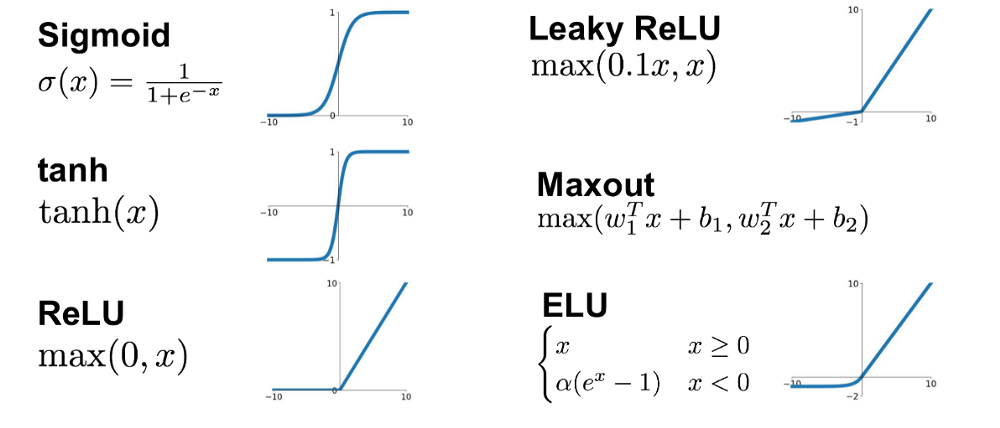
\includegraphics[width=0.80\textwidth] {./Figuras/mc_ai/activation_functions.png}
        	
        	\caption{Funções de Ativação} \subcaption*{Fonte: \cite{MCAI}, https://mc.ai/complete-guide-of-activation-functions/}} \label{fig:activation_functions}
        \end{figure}
	    \subsubsection{Para a entrada e camadas ocultas}
    	    A função ReLu é simples e eficiente para a aplicação nos experimentos, visto que na fase feed-forward tem efeito parecido com a função identidade, e na fase feed-backward durante o reajuste dos pesos pelo otimizador, produz efeito degrau zerando valores negativos e sendo adequada na aplicação do domínio de entrada deste trabalho, visto que todas as variáveis endógenas e exógenas não possuem valores negativos.
    	\subsubsection{Para a saída}
    	    Para os valores previstos a função escolhida é a linear, pois na fase feed-backward do reajuste dos pesos pelo algoritmo de treino backpropagation, a derivada da função linear se torna zero, mantendo a execução do algoritmo de treino transformando apenas os valores de entrada e valores das camadas ocultas das redes, sem interferir no valor de saída.
%TODO-T: FIGURA 25 ESTORANDO MARGEM NO TITULO    	
    \subsection{Otimizador}
        \begin{figure}[H]
        	\center{
        		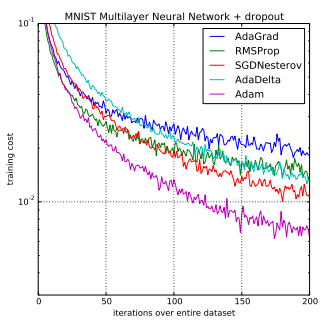
\includegraphics[width=0.80\textwidth]
        		{./Figuras/MLM/optimizers.png}
        	
        	\caption{Comparison of Adam to Other Optimization Algorithms Training a Multilayer Perceptron} \subcaption*{Fonte : \cite{MLM} https://machinelearningmastery.com/adam-optimization-algorithm-for-deep-learning/}} \label{fig:otimizadores}
        \end{figure}
        Para este trabalho foi escolhido o otimizador ADAM no treino de backpropagation.
        A vantagem deste otimizador é a fusão das melhores características de 2 otimizadores :\newline 
         Momenum e RMSProp. \newline
        O Momentum acelera o reajuste dos pesos em busca dos erros globais mínimos.\newline
         O RMSProp impede a busca na direção das oscilações.\newline
         Adam ou Adaptive Moment otimization combina estas 2 heurísticas.
        O coeficiente de aprendizado escolhido para o otimizador, ou conhecido como "learning rate", foi definido para a constante alpha, com valor 0.001.
        Esta constante tem produzido resultados positivos em problemas de forecast (predições) de acordo com o artigo fundamentado em \cite{MLM}.

    \section{Teste e Métricas}
       A principal métrica de avaliação dos modelos, é a Raiz do Erro Quadrático Médio, obtido pela chamada de função "mean\_squared\_error"\ do framework Tensorflow.Keras utilizado para a modelagem,treino e predição dos modelos de redes neurais.
       
        O coeficiente de correlação de Pearson, obtido pela biblioteca scipy na chamada de função \"scipy.stats.pearsonr(true,pred)"\ e o coeficiente "chi-quadrado" definido como $R^2$ obtido na chamada de função \"scipy.stats.linregress"\ foi utilizado nas etapas de teste para avaliar a proximidade das predições do modelo com o comportamento real de consumo (Se acompanha as quedas e subidas de consumo ao longo do tempo).\newline
       
        Documentou-se, para trabalhos futuros, outras métricas estatísticas obtidas por esta chamada de função como os valores de slope, intercept, p\_value e std\_err.\newline
       
        A chamada de função sns.regplot(x=arr\_true,y=arr\_pred,data=df) da biblioteca seaborn  retorna um gráfico scatter dos valores preditos e reais para a avaliação dos erros, médias e tendencia de previsão.\newline 
       
       Avaliou-se também os erros positivos e negativos entre os valores previstos e reais, para representar quantas refeições seriam descartadas e quantas estariam em falta se a produção de refeições fosse de acordo com as predições do modelo.
       
  % ----------------------------------------------------------
  % \chapter{METODOLOGIA}
  % ----------------------------------------------------------